\documentclass[UTF8,fontset=ubuntu]{ctexart}
\usepackage{tikz}
\usetikzlibrary{trees}
\begin{document}
% 树状图,section 76
% update 2025-04-15
\begin{tikzpicture}
    \coordinate
      child {}
      child {
        child {}
	child {}
      };
\end{tikzpicture}\\\vspace{1cm}

\begin{tikzpicture}
    \node {}
      child { node{}
        child {node{}}
        child {node{}}
      };
\end{tikzpicture}\\\vspace{1cm}

\begin{tikzpicture}
    \node {实数}
      child { node {无理数}}
      child { node {有理数}
        child {node {整数}}
        child {node {分数}}
      };
\end{tikzpicture}\\\vspace{1cm}

% 相关参数:
%   1.grow - 在指定延伸方向的前提下,将child按逆时针方向排列. 可选延伸方向列表:
%     [1]down/up/left/right - 分别为向下/上/左/右方向延伸. 默认为down
%     [2]north/south/west/east/north west/north east/south west/south east - 分别为北/南/西/东/西北/东北/西南/东南方向延伸
%     [3]角度值 - 向指定角度方向延伸. x轴正向为0度
%   2.grow' - 类似于grow,将child按顺时针方向排列
%   3.level distance - 父节点与子节点(节点中央)之间的距离
%   4.sibling distance - 兄弟节点(节点中央)之间的距离
%   5.<color> - 给连线和节点配置颜色
% ** 在\begin{tikzpicture}[<option>]配置,作用于全局,level <num>/.style适用于指定层级节点
% ** 在child[<option>]配置,则作用于当前节点和后续子孙节点
% ** 在node[<option>]配置,则只作用于当前node,every node/.style适用于所有node
% ** edge from parent/.style用于指定父节点到子节点之间的线条
\begin{tikzpicture}[font=\footnotesize,grow=right,level 1/.style={sibling distance=6em},level 2/.style={sibling distance=1em},level distance=5cm]
\node {Computational Complexity} % root
  child { node {Computational Problems}
    child { node {Problem Measures} }
    child { node {Problem Aspects} }
    child { node {Problem Domains} }
    child { node {Key Problems} }
  }
  child { node {Computational Models}
    child { node {Turing Machines} }
    child { node {Random-Access Machines} }
    child { node {Circuits} }
    child { node {Binary Decision Diagrams} }
    child { node {Oracle Machines} }
    child { node {Programming in Logic} }
  }
  child { node {Measuring Complexity}
    child { node {Complexity Measures} }
    child { node {Classifying Complexity} }
    child { node {Comparing Complexity} }
    child { node {Describing Complexity} }
  }
  child { node {Solving Problems}
    child { node {Exact Algorithms} }
    child { node {Randomization} }
    child { node {Fixed-Parameter Algorithms} }
    child { node {Parallel Computation} }
    child { node {Partial Solutions} }
    child { node {Approximation} }
  };
\end{tikzpicture}\\\vspace{1cm}

% 相关参数:
%   7.grow cyclic - 沿圆方向拓展. 需要trees tikz库
%   8.sibling angle - 当前节点到兄弟节点的角度,配合grow cyclic使用. 需要trees tikz库
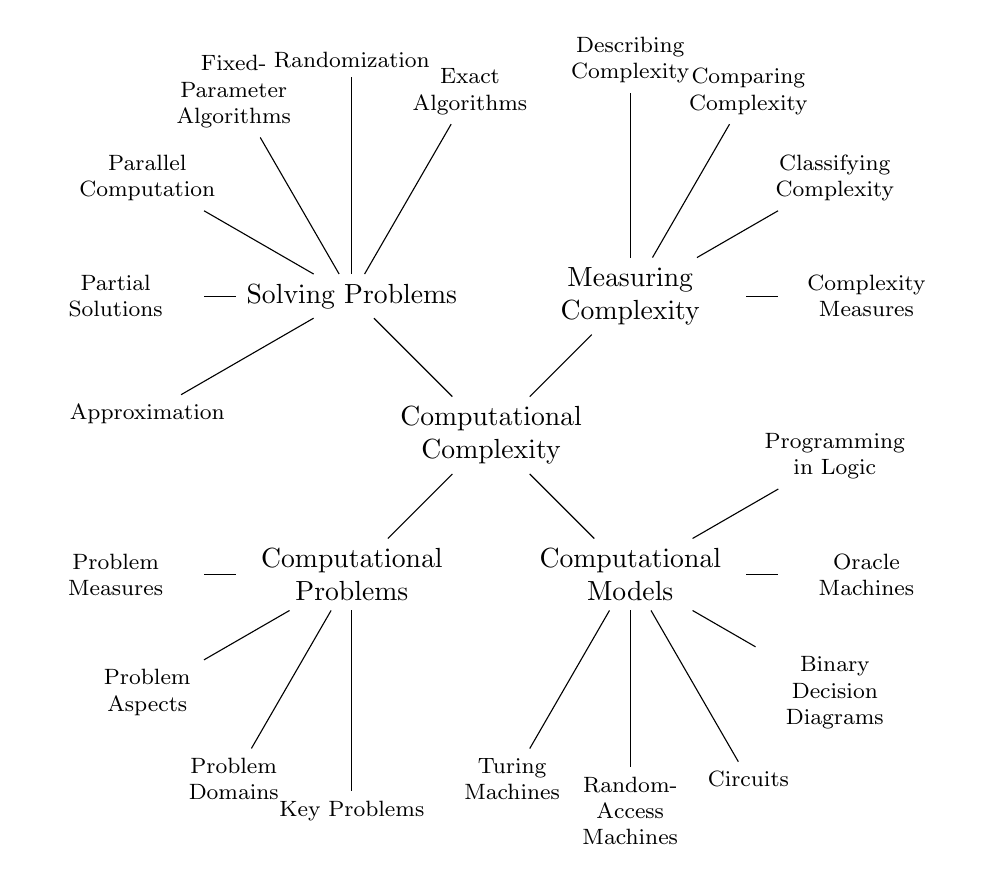
\begin{tikzpicture}[align=flush center,text width=2.7cm,grow cyclic,level 1/.style={level distance=2.5cm,sibling angle=90},level 2/.style={text width=2cm,level distance=3cm,font=\footnotesize,sibling angle=30}]
\node {Computational Complexity} % root
  child { node {Computational Problems}
    child { node {Problem Measures} }
    child { node {Problem Aspects} }
    child { node {Problem Domains} }
    child { node {Key Problems} }
  }
  child { node {Computational Models}
    child { node {Turing Machines} }
    child { node {Random-Access Machines} }
    child { node {Circuits} }
    child { node {Binary Decision Diagrams} }
    child { node {Oracle Machines} }
    child { node {Programming in Logic} }
  }
  child { node {Measuring Complexity}
    child { node {Complexity Measures} }
    child { node {Classifying Complexity} }
    child { node {Comparing Complexity} }
    child { node {Describing Complexity} }
  }
  child { node {Solving Problems}
    child { node {Exact Algorithms} }
    child { node {Randomization} }
    child { node {Fixed-Parameter Algorithms} }
    child { node {Parallel Computation} }
    child { node {Partial Solutions} }
    child { node {Approximation} }
  };
\end{tikzpicture}\\\vspace{1cm}

% 相关参数:
%   9.grow via three points={one child at (<coordinate_x>) and two children at (<coordinate_y>) and (<coordinate_z>)}
%     通过三个坐标点,确定树的子节点位置. 需要trees tikz库
%     当只有一个子节点时,子节点坐标为coordinate_x
%     当只有两个子节点时,子节点坐标为coordinate_y和coordinate_z
%     当包含三个子节点或以上时,子节点坐标计算公式x+(n-1)*(y-x)+(c-1)(z-y). 其中, n为子节点总数,c为当前子节点的号码(计数从1起始)
%     ** 所有数量子节点都符合公式,x/y/z位置关系y x z
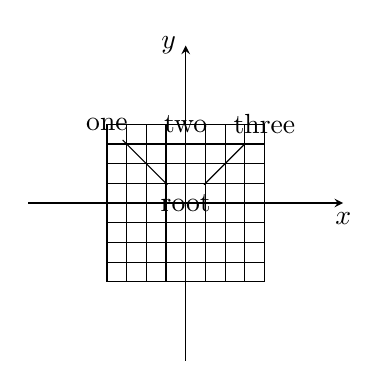
\begin{tikzpicture}[>=stealth,grow via three points={one child at (0,1) and two children at (-0.5,1) and (0.5,1)}]
    \draw[->] (-2,0) -- (2,0) node[below]{$x$};
    \draw[->] (0,-2) -- (0,2) node[left]{$y$};
    \foreach \x in {-1,-0.75,...,1}{
      \draw (\x,-1) -- (\x,1);
      \draw (-1,\x) -- (1,\x);
    }
    \node at (0,0) {root}
      child {node {one}}
      child {node {two}}
      child {node {three}};
\end{tikzpicture}\vspace{1cm}

% 相关参数:
%   10.clockwise from=<angle>
%     以指定角度开始,并顺时针沿圆环绕
%     使用sibling angle指定子节点之间的偏转角度
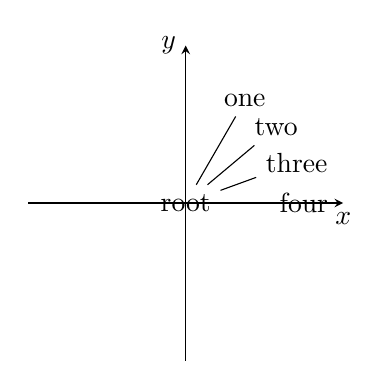
\begin{tikzpicture}[>=stealth,clockwise from=60,sibling angle=20]
    \draw[->] (-2,0) -- (2,0) node[below]{$x$};
    \draw[->] (0,-2) -- (0,2) node[left]{$y$};
    \node at (0,0) {root}
      child {node {one}}
      child {node {two}}
      child {node {three}}
      child {node {four}};
\end{tikzpicture}\vspace{1cm}

% 相关参数:
%   11.counterclockwise from=<angle>
%     以指定角度开始,并逆时针沿圆环绕
%     使用sibling angle指定子节点之间的偏转角度
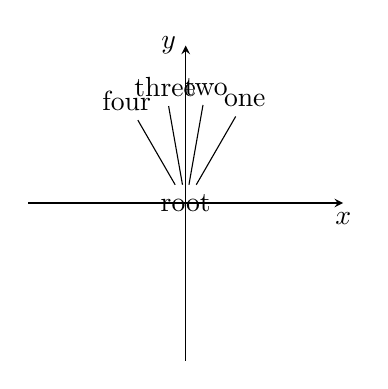
\begin{tikzpicture}[>=stealth,counterclockwise from=60,sibling angle=20]
    \draw[->] (-2,0) -- (2,0) node[below]{$x$};
    \draw[->] (0,-2) -- (0,2) node[left]{$y$};
    \node at (0,0) {root}
      child {node {one}}
      child {node {two}}
      child {node {three}}
      child {node {four}};
\end{tikzpicture}\vspace{1cm}

% 相关参数:
%   12.edge from parent fork down、edge from parent fork up、edge from parent fork left、edge from parent fork right
%     指定从父节点到子节点的连线方式为折线,向指定方向拓展
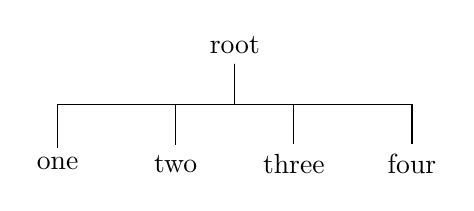
\begin{tikzpicture}[>=stealth,edge from parent fork down]
    \node at (0,0) {root}
      child {node {one}}
      child {node {two}}
      child {node {three}}
      child {node {four}};
\end{tikzpicture}
\end{document}
